\chapter{神经网络处理器编译器测试流程}
\section{神经网络处理器的整体架构}
神经网络处理器是针对大数据量神经网络相关计算设计的专用加速硬件。神经网络加速器提供的高效运算包括了卷积,池化,激活,基本矩阵乘法,归一化等操作。通过专门设计的特有物理结构和指令集,可以实现高效的与神经网络相关的计算。物理结构包括特有的物理存储结构和计算核心结构。指令集则是指一系列特殊定义的用于操作底层硬件的二进制编码的集合。神经网络加速器可以是处理器之外的专用加速设备。神经网络加速器可以以不同的形式与现有的通用处理器进行集成,形成神经网络加速系统。按照与现有通用处理器耦合程度(从紧耦合至松耦合),可行的集成方式至少包括以下几种:1. 将神经网络加速器作为CPU 的功能部件,集成到CPU 的流水线中;2. 将神经网络加速器与CPU 集成到系统芯片SoC 中;3. 神经网络加速器设计为兼容PCIe 协议的板块,通过PCIe与CPU 进行连接。

在我们现阶段的处理器实现过程中,我们所采用的方式,是通过PCI Express高速总线与CPU 实现互联。PCIe 总线速度快,并且在现在的各种处理器互联中广泛运用。

\begin{figure}[!htbp]
\centering
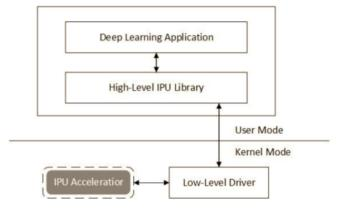
\includegraphics[width=12cm]{IPU.jpg}
\caption{神经网络处理器的架构}
\label{fig:IPU}
\end{figure}

在本文测试过程中,使用的已实现的神经网络处理器架构图如\autoref{fig:IPU}所示。

在用户的应用程序中,为了调用神经网络处理器去准确方便的完成神经网络相关计算,一套稳定可靠的应用程序接口也是不可或缺的。接下来我们将详细介绍神经网络处理器的软件架构。

\section{神经网络处理器的软件架构}
在阐明验证思路之前,我们应首先来熟悉一下神经网络处理器的软件架构, 如\autoref{fig:Software stock}所示,神经网络处理器的软件部分自上而下主要分成如下几个层次:

1.User Program:上层应用,即程序员基于编程框架。定义特定的神经网络结构来实现特定的神经网络功能。

2.Framework:编程框架,相当于连接的桥梁。例如(Caffe、TensorFlow),为用户提供神经网络基本操作,减轻程序员的编程负担,是一种编程工具。

3.runtime library:IPU库是一个屏蔽掉底层硬件,编译器、启动程序的具体信息,对上层编程框架提供神经网络原子(即神经网络的某一层,这是神经网络最基本的组成单元)操作的编程接口的系统软件,它具有内存分配和释放、基本运算、指令生成和数据传输等功能。

IPU库集成封装了神经网络基本的运算操作,如Conv(卷积)、Pooling(池化)、Active(激活函数)、BatchNorm(批规范化)、FullyConnected(全连接)等等常见操作,还有更详细矩阵的数学运算如乘法、加法、减法、缩放等等,这样可以直接调用IPU 的接口,就能直接实现神经网络,同时将优化IPU 的工作封装在IPU 库这一个层次中,而不用直接向应用程序展露。

4.driver、compile:编译器,将上层的库传来的指令描述符按照神经网络处理器的指令集翻译成能接受的机器指令。
驱动:对上层库提供调用底层硬件最基本的操作支持,例如读取数据、启动关闭、读取寄存器等。

5.hardware 硬件:即神经网络处理器(DaDianNao)

\begin{figure}[!htbp]
\centering
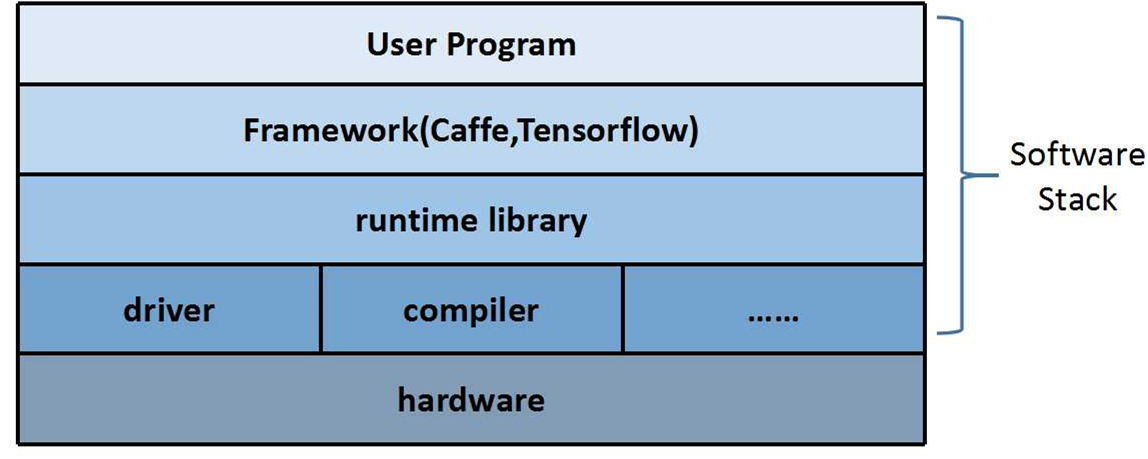
\includegraphics[width=12cm]{Software_stock.jpg}
\caption{神经网络处理器的软件架构}
\label{fig:Software stock}
\end{figure}

\section{测试流程}
在还没有神经网络处理器测试框架的时候,我们曾采取随机生成单个指令的方式来进行验证。然而,由于神经网络处理器指令粒度较大,随机指令无法覆盖到实际使用需求的指令序列,所以需要实际的使用者,也就是编译器生成的指令来做二次审查。这实际上也对应了传统软件测试方法中基于模型测试的思想。

在我们的测试过程中,需要对变量进行控制,由于我们需要测试的是神经网络处理器的编译器,因此主要关注的是库(runtime library)以及编译器(compiler)的正确性。

对于神经网络处理器编译器的验证流程,可以概括为如下几个步骤,首先,生成包含有网络参数与结构信息的配置文件prototxt 。接着,根据prototxt调用caffe提供的接口生成具有训练参数的神经网络模型caffe\underline{ }modrel,然后调用caffe框架,经过一系列的内存分配,指令生成的操作后,调用库的接口,获得神经网络处理器结果,将这个结果caffe中生成的cpu结果进行比对,以达到验证目的。

接下来将详细论述流程的步骤。
\subsection{protext的生成}
要运行caffe,首先需要先创建一个模型(model),caffe里自带了不少常用的神经网络模型,而一个模型由多个层(layer)构成,每一个层又包含多个参数,每一个层的参数都定义在caffe.proto这个文件内。因此,想要生成一个可以用于测试的模型,我们首先得生成一个符合结构要求并含有参数定义的prototxt。

我们自己编写了一套随机网络生成器,通过这个随机网络生成器,我们可以根据用户的需求,生成结构随机,参数随机且具有正确合理的连接方式的神经网络。同时,这个生成器也可以根据用户需求,生成包含有指定层序列、甚至是结构固定的网络,同时,我们也搭建了一个数据库,分三个层次将一些网络的样例加入数据库中。关于随机网络生成器的细节将在第三章详细概述。

\subsection{caffe\underline{ }model的创建}
在得到了包含有网络结构及参数的配置文件prototxt后,我们调用caffe提供的caffe\underline{ }param接口(caffe\underline{ }param是caffe提供的一个记录网络结构与权值并能直接生成caffe\underline{ }model的类),以此初始化一个Net类,在Net中我们将权值初始化,再赋以随机权值传回param类中,而后net\underline{ }param便可以直接将网络结构以及权值写入caffe\underline{ }model中,我们就生成一个具有随机权值的真实网络。

我们先用caffe调用cpu计算数据通过这个网络的结果,而后再调用我们的神经网络处理器。

\subsection{caffe重载}
caffe是一个快速的深度学习框架,现在只能调用cpu与gpu进行计算。因此,为了让caffe能够调用神经网络处理器进行运算,我们对caffe进行了移植,在框架下加入对神经网络处理器硬件的支持。把原来的cpu操作,重载成为神经网络处理器的指令,成为库能接受的操作和运算。

从实现上来看,即将操作的xxx\underline{ }Forward\underline{ }cpu改写为支持神经网络处理器运算的xxx\underline{ }Forward\underline{ }ipu。同时,我们也在内存调度与空间管理等细节上进行了完善,使得caffe可以支持神经网络处理器的运算。

\subsection{caffe调用库的过程}
\begin{figure}[!htbp]
\centering
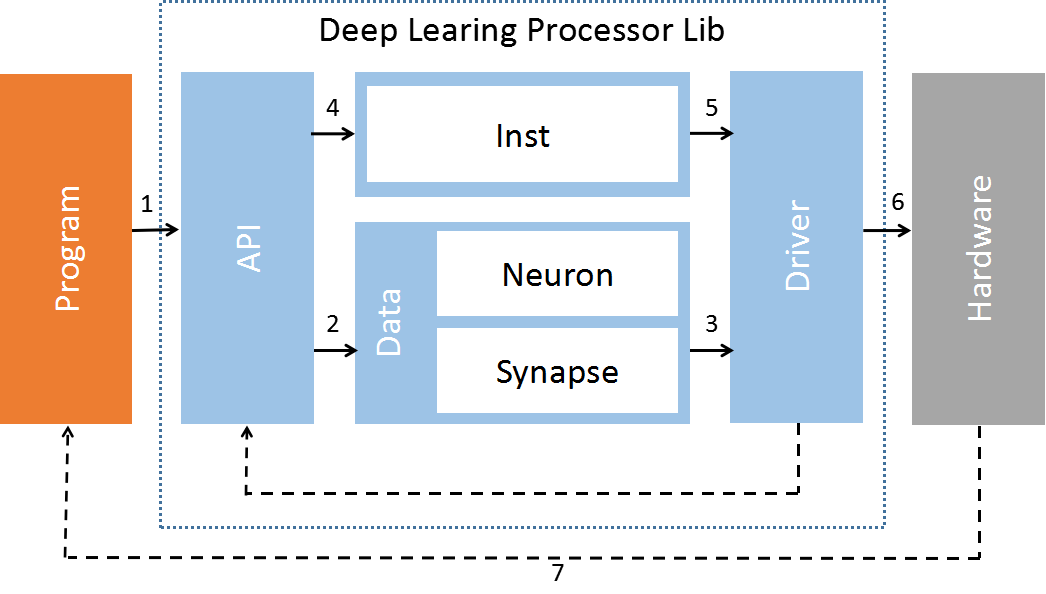
\includegraphics[width=12cm]{DLP1.png}
\caption{库的执行模型}
\label{fig:DLP model}
\end{figure}
caffe运行神经网络处理器的流程如\autoref{fig:DLP model}所示,库的调用大致分为以下流程:

1.初始化神经网络处理器的库

2.声明和设置描述符(tensor描述符,算法描述符,操作描述符)

3.准备数据(nalloc CPU数据和神经网络处理器数据,CPU到神经网络处理器的数据拷贝)

4.IPU运算(xxx\underline{ }Forward函数调用)

5.读取结果

至此,我们已经得到了神经网络处理器结果,将这个结果caffe中生成的cpu结果进行比对,便可以达到验证目的。
\section{测验工作的进程}
对于随机网络生成器来说,现在已经能支持包括卷积,池化,激励等层在内的18种层类型的生成。依靠神经网络处理器测验框架,我们基本完成了库的测试工作,保证了寒武纪系列神经网络处理器编译器的的正确性及可靠性。
\section{本节总结}
本节首先先从神经网络处理器的整体构架说起,而后详细的介绍了神经网络处理器的软件构架并着重点出了我们验证的主要目标。接着,从prototxt的生成到caffemodel的建立,再到caffe的的重载直到最后指令的调用,层层深入,详细介绍了神经网络处理器编译器的验证流程,并简要介绍了使用该测验框架后,测验工作的进程。